\begin{table}[t!]
\centering

\caption{Architectural comparison of agent methods with objective complexity metrics. Computational complexity measured in terms of LLM calls, coordination overhead, and parallelization potential.}
\label{tab:agent_methods_complexity}

{\fontsize{7}{8.5}\selectfont
\begin{tabularx}{\textwidth}{p{2.4cm} >{\centering\arraybackslash}X >{\centering\arraybackslash}X >{\centering\arraybackslash}X >{\centering\arraybackslash}X >{\centering\arraybackslash}X}
\toprule
\textbf{Characteristic} & \textbf{SAS} & \makecell{\textbf{MAS} \\ (\textbf{Independent})} & \makecell{\textbf{MAS} \\ (\textbf{Decentralized})} &
\makecell{\textbf{MAS} \\ (\textbf{Centralized})}  & \makecell{\textbf{MAS} \\ (\textbf{Hybrid})} \\ \hline
\multirow{1}{*}[15pt]{\vspace{3em}\textbf{Interaction Type}}
& 
\includegraphics[width=0.65cm]{imgs/sas.pdf}
& 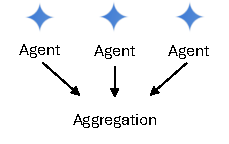
\includegraphics[width=2.3cm]{imgs/mas_independent.pdf}
& 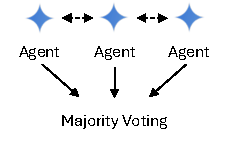
\includegraphics[width=2.4cm]{imgs/mas_decentralized.pdf}
& 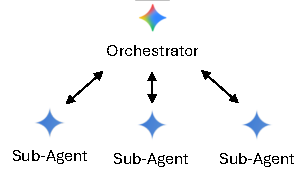
\includegraphics[width=2.65cm]{imgs/mas_centralized.pdf}
& 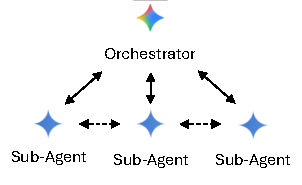
\includegraphics[width=2.65cm]{imgs/mas_hybrid.pdf} \\
\textbf{LLM Calls} & $O(k)$ & $O(nk) + O(1)$ & $O(dnk) + O(1)$ & $O(rnk) + O(r)$ & $O(rnk) + O(r) + O(p)$ \\
\textbf{Sequential Depth} & $k$ & $k$ & $d$ & $r$ & $r$ \\
\textbf{Comm. Overhead} & $0$ & $1$ & $d \cdot n$ & $r \cdot n$ & $r \cdot n + p \cdot m$ \\
\textbf{Parallelization Factor} & $1$ & $n$ & $n$ & $n$ & $n$ \\
\textbf{Memory Complexity} & $O(k)$ & $O(n \cdot k)$ & $O(d \cdot n \cdot k)$ & $O(r \cdot n \cdot k)$ & $O((r + p) \cdot n \cdot k)$ \\
\textbf{Coordination} & Sequential & Parallel + Synthesis & Sequential Debate & Hierarchical & Hierarchical + Peer \\
\textbf{Consensus} & - & Synthesis & Debate & Orchestrator & Orchestrator \\
\bottomrule
\end{tabularx}
}

\vspace{-0.3em}
\begin{flushleft}
{\fontsize{10}{11}\selectfont
\textbf{*} $k$ = max iterations per agent, $n$ = number of agents, $r$ = orchestrator rounds, $d$ = debate rounds, $p$ = peer communication rounds, $m$ = average peer requests per round. Communication overhead counts inter-agent message exchanges. Independent offers maximal parallelization with minimal coordination. Decentralized uses sequential debate rounds. Hybrid combines orchestrator control with directed peer communication.
}
\end{flushleft}

\end{table}
  
  

\section{Experiments \& Results}
\label{sec:results}

To establish quantitative scaling principles for agentic systems, we investigate three research questions:

\noindent\textbf{RQ1.} What factors determine agent system's performance (e.g., model capability, coordination architecture, task properties, their interactions)? \textcolor{black}{We systematically vary each factor across 260 configurations to quantify their individual and joint contributions.}

\noindent\textbf{RQ2.} Under what conditions does inter-agent coordination improve or degrade agent system's performance? We examine how task structure (e.g., decomposability, tool complexity, sequential dependencies) moderates the effectiveness of different architectures.

\noindent\textbf{RQ3.} Can we derive quantitative scaling principles that predict best agent architecture for a given task from measurable properties? We fit a regression model using empirical coordination metrics to test whether continuous properties outperform categorical architecture labels in explaining performance variance.



\begin{figure}[ht!]
  \centering
  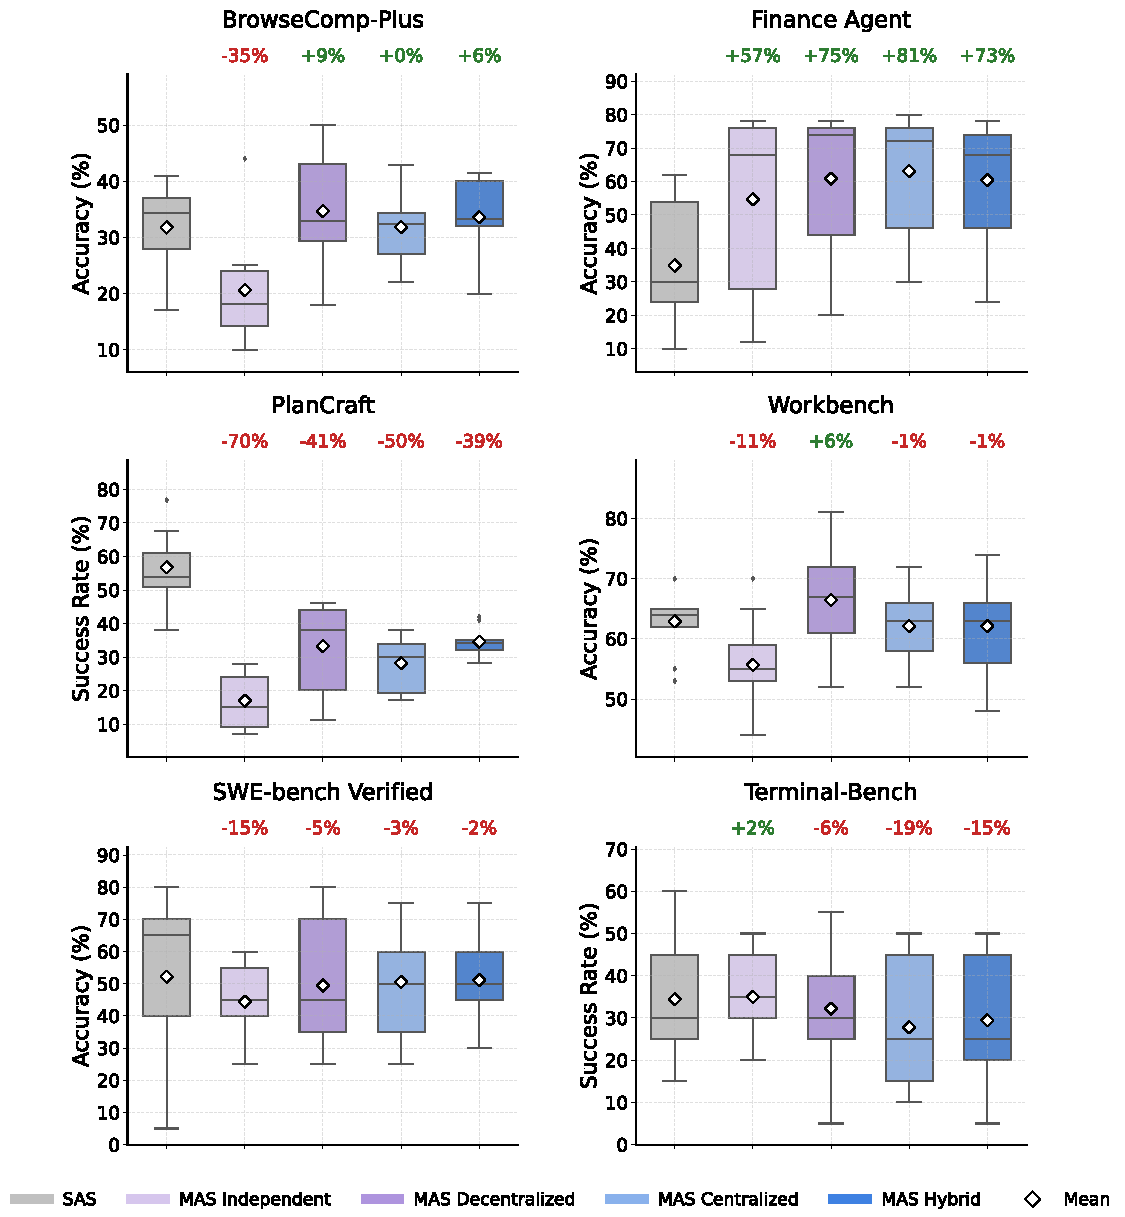
\includegraphics[width=0.9\textwidth]{imgs/boxplots_v4.pdf}
  \caption{
  \textcolor{black}{\textbf{Comparative performance of agent systems across six agentic benchmarks reveals highly task-dependent scaling dynamics.}} \textcolor{black}{Box plots show distribution of performance (0--100\%).} Percentage annotations represent \textit{relative} improvement/degradation compared to SAS baseline: $(\text{mean}_{\text{MAS}} - \text{mean}_{\text{SAS}})/\text{mean}_{\text{SAS}} \times 100\%$. SAS serves as the reference baseline (shown without percentage annotation).
  \textbf{(a)} BrowseComp-Plus shows polarized results, with independent agents catastrophically underperforming relative to SAS (-35\%) while more structured coordination achieves modest gains. \textbf{(b)} Finance Agent demonstrates the strongest multi-agent benefits, with all MAS architectures substantially outperforming SAS (from +57\% to +80.8\%). \textbf{(c)} PlanCraft exhibits consistent degradation across all MAS variants (from -70\% to -39\%). \textbf{(d)} Workbench shows marginal effects (from -11 to +6\%). \textcolor{black}{\textbf{(e)} SWE-bench Verified shows slight degradation across all MAS architectures (from -15\% to -2\%), consistent with high single-agent baselines ($>$45\%) for most models. \textbf{(f)} Terminal-Bench shows mixed results: Independent achieves marginal gains (+2\%) while Centralized degrades (-19\%), reflecting the low tool count (2 tools) where coordination overhead is less justified.} 
  }
  \label{fig:boxplots}
  \end{figure}

  
  
  
  
\subsection{Setup}
  
\paragraph{Benchmarks.}
\textcolor{black}{We conducted 260 experiments across six benchmarks spanning deterministic to open-world task structures: \textbf{Workbench} (deterministic code execution and tool use with objective pass/fail criteria), \textbf{Finance Agent} (multi-step quantitative reasoning and risk assessment), \textbf{PlanCraft} (spatiotemporal planning under constraints), \textbf{BrowseComp-Plus} (dynamic web navigation, information extraction, and cross-page synthesis), \textbf{SWE-bench Verified} (real-world software engineering; GitHub issue resolution with 7 tools including bash, file editing, and test execution), and \textbf{Terminal-Bench} (diverse CLI tasks spanning system administration, security, and ML training; 2 tools). BrowseComp-Plus, Finance Agent, PlanCraft, and Workbench each contribute 45 configurations (9 models $\times$ 5 architectures); SWE-bench Verified and Terminal-Bench each contribute 40 configurations (8 models $\times$ 5 architectures, as Claude Sonnet 3.7 is deprecated). BrowseComp-Plus, Finance Agent, PlanCraft, and Workbench use 50--100 instances per configuration; SWE-bench Verified and Terminal-Bench use 20-instance subsets due to the computational cost of Docker-based evaluation (see Table~\ref{tab:s6_bootstrap} for bootstrap confidence intervals). The tool-count range spans $\{2,3,4,5,7,16\}$ across all six benchmarks.} BrowseComp-Plus exhibits the highest performance variability across experimental configurations (coefficient of variation $\sigma/\mu= 0.32$ computed across all 45 BrowseComp-Plus runs spanning architectures and model families, with Anthropic models contributing substantial variance due to lower absolute performance, where $\sigma$ is the standard deviation of success rates and $\mu$ is the mean success rate). By comparison, Workbench (CV=0.12), Finance Agent (CV=0.18), and PlanCraft (CV=0.21) show lower variability, indicating more stable performance across configurations. 
  
  
\paragraph{LLMs and Intelligence Scaling.} We evaluate three LLM families across multiple model sizes, spanning externally standardized Intelligence Index values from 42 to 71 (a composite capability score integrating reasoning, coding, and knowledge benchmarks; see Appendix \ref{sec:appendix-intelligence-index}):
\begin{itemize}[leftmargin=1.5em, topsep=2pt, itemsep=1pt]
    \item \textbf{OpenAI:} \textit{GPT-5-nano, GPT-5-mini, GPT-5}
    \item \textbf{Google:} \textit{Gemini-2.0 Flash, Gemini-2.5 Flash, Gemini-2.5 Pro}
    \item \textbf{Anthropic:} \textit{Claude Sonnet 3.7, Claude Sonnet 4, Claude Sonnet 4.5}
\end{itemize}
\textcolor{black}{Claude Sonnet 3.7 was deprecated by Anthropic in February 2026 and is therefore unavailable for SWE-bench Verified and Terminal-Bench. On these two benchmarks, the Anthropic family includes Claude Sonnet 4 and Claude Sonnet 4.5, while the OpenAI and Google families remain unchanged, yielding 8 models per benchmark and a total of $N{=}260$ configurations.}
Strong consistency across families validates that coordination scaling follows model-agnostic principles: the maximum difference in architecture-specific scaling slopes between any two LLM families is $\Delta_{\max} = 0.023$ (computed as $\max_{i,j}|\hat{\beta}_{\text{arch},i} - \hat{\beta}_{\text{arch},j}|$ across families $i,j \in \{\text{OpenAI, Google, Anthropic}\}$), with coefficient of variation CV $< 0.02$ across families. To ensure computational fairness, we matched maximum total iterations between MAS and SAS systems: MAS configurations received equal computational budget through parallel agent processing (smaller per-agent iterations for $n$-agent teams), while SAS received proportionally more reasoning rounds to compensate for lack of parallel deliberation.
  
\paragraph{Agent Architectures and Complexity.}
We tested five coordination topologies: Single-Agent System (SAS) and four Multi-Agent System (MAS) variants: Independent, Centralized, Decentralized, and Hybrid. Rather than attempting exhaustive coverage of all possible architectures, we selected these four MAS configurations to form a structured ablation over two key coordination dimensions: 
(i) \textit{orchestrator presence} (hierarchical control vs. flat structure), and (ii) \textit{peer communication} (direct sub-agent interaction vs. isolated execution). Independent isolates pure ensemble effects without any inter-agent communication; Centralized introduces hierarchical verification through an orchestrator bottleneck; Decentralized enables 
peer-to-peer information fusion without hierarchy; and Hybrid combines both mechanisms (see Table \ref{tab:agent_methods_complexity} for formal complexity characterization). This design enables controlled
attribution of performance differences to specific coordination
mechanisms rather than generic ``multi-agent'' effects. Coordination complexity is parameterized by communication overhead: the total number of inter-agent message exchanges required per task, yielding empirical values ranging from 0\% (SAS) to 515\% (Hybrid), with Independent at 58\%, Decentralized at 263\%, and Centralized at 285\% relative to the single-agent baseline (see Table~\ref{tab:coord_metrics}).
  
\paragraph{Metrics and Validation.}
Primary outcome is task success/accuracy (domain-dependent: factual correctness for Finance Agent, task completion for Workbench, goal satisfaction for PlanCraft, page synthesis accuracy for BrowseComp-Plus). Secondary metrics include: (i) factual error rate $E$ via domain-specific validators (Cohen's $\kappa$ \citep{cohen1960coefficient}: Finance Agent $= 0.91$, Workbench $= 0.89$, PlanCraft $= 0.87$, BrowseComp-Plus $= 0.88$; exceeding 0.80, indicating strong inter-rater reliability); (ii) information gain $\Delta \mathcal{I}$ from pre- vs.\ post-coordination uncertainty proxies (see Eq.~\ref{eq:info_gain}); (iii) token-overlap structure across agent rationales, labeling tokens as unique (appearing in exactly one agent), shared (two or more agents), or contradictory (semantic opposition detected when BERTScore similarity $< 0.3$ between assertion pairs, i.e., $1 - \text{BERTScore} > 0.7$, following the dissimilarity threshold established by \citet{zhang2019bertscore}); (iv) efficiency metrics including success per 1,000 tokens and cost-normalized performance. All metrics are normalized per reasoning turn and per token to enable cross-architecture comparison. We select coordination metrics based on two criteria: (i) direct measurability from experimental traces without requiring ground-truth labels beyond task success, and (ii) coverage of distinct aspects of coordination--performance relationships identified in prior work \citep{cemri2025multi}. We excluded metrics requiring subjective human annotation (e.g., solution creativity) or those exhibiting high collinearity with included measures (e.g., total message count correlates $r > 0.92$ with overhead). Variance inflation factor (VIF) analysis confirmed no severe multicollinearity among retained predictors (all VIF $< 5$). Specifically:

\begin{itemize}[leftmargin=1.5em, topsep=2pt, itemsep=1pt]

\item \textbf{Coordination overhead} $O = (T_{\text{MAS}} - T_{\text{SAS}})/T_{\text{SAS}} \times 100\%$: captures computational cost, identified as a primary bottleneck in production multi-agent deployments.

\item \textbf{Message density} $c$ (inter-agent messages per reasoning turn): quantifies communication intensity, a key factor in coordination scaling.

\item \textbf{Redundancy rate} $R$ (mean cosine similarity of agent output embeddings): measures agent agreement, relevant for ensemble-based error correction.

\item \textbf{Coordination efficiency} $E_c = S/(T/T_{\text{SAS}})$ (success normalized by relative turn count): normalizes success by cost for deployment decisions.


\item \textbf{Error amplification} $A_e^{\text{trace}}$ (trace-level error propagation factor, estimated from execution-trace token analysis): quantifies how coordination failures compound through agent interactions. The complementary task-level metric $A_e^{\text{task}} = E_{\text{MAS}}/E_{\text{SAS}}$ is defined in Section~\ref{sec:methods}.
\end{itemize}
  
\subsection{Main Results}
\label{subsec:main_results}
  
\paragraph{MAS exhibits domain-dependence with architectural variation.}
Multi-agent systems show highly variable performance across task domains, depending on problem structure and architectural choices. On Finance Agent, MAS achieve substantial improvements: Centralized reaches \textbf{+80.8\%} (mean 0.631 vs.\ SAS 0.349), Decentralized achieves \textbf{+74.5\%} (0.609), and Hybrid reaches \textbf{+73.1\%} (0.604), driven by opportunities for distributed financial reasoning across multiple agents. On Workbench, multi-agent systems show minimal gains: Decentralized achieves \textbf{+5.6\%} (0.664 vs.\ SAS 0.629), while Centralized and Hybrid both slightly underperform at \textbf{-1.2\%}. On BrowseComp-Plus, improvements remain modest: Decentralized achieves \textbf{+9.2\%} (0.347 vs.\ SAS 0.318), with Centralized essentially flat at \textbf{+0.2\%}. Critically, PlanCraft exhibits universal performance degradation 
across all multi-agent architectures. Centralized declines to 
$-50.3$\% (0.282 vs.\ SAS 0.568), Decentralized to $-41.5$\% (0.332), Hybrid to $-39.1$\% (0.346), and Independent to $-70.0$\% (0.170). To understand this
contrast between Finance Agent's gains and PlanCraft's degradation, we examined execution traces from both domains. In PlanCraft, efficient single-agent trajectories follow direct execution paths. For example, crafting a \texttt{diorite\_wall}:
\begin{quote}
\texttt{Turn 1: search("diorite\_wall") $\rightarrow$ Recipe: 6 diorite in 2x3}\\
\texttt{Turn 2: move(diorite $\rightarrow$ crafting\_grid)}\\
\texttt{Turn 3: craft $\rightarrow$ Task complete}
\end{quote}
In contrast, centralized multi-agent systems decompose inherently sequential tasks into artificial subtasks:
\begin{quote}
\texttt{Agent 1: Research recipe} (redundant, since lookup is instantaneous)\\
\texttt{Agent 2: Check inventory} (redundant, since state is visible to all)\\
\texttt{Agent 3: Execute crafting} (the only necessary step)
\end{quote}
This unnecessary decomposition generates substantial coordination messages on average for tasks requiring only a few execution steps, consuming token budget on coordination rather than reasoning. Conversely, Finance Agent trajectories demonstrate when coordination provides genuine value. Single-agent execution exhibits sequential bottlenecks:
\begin{quote}
\texttt{Turn 1: web\_search("merger news") $\rightarrow$ Surface results}\\
\texttt{Turn 2: edgar\_search("filings") $\rightarrow$ Limited depth}\\
\texttt{Turn 3--7: Sequential exploration with insufficient breadth}
\end{quote}
Centralized coordination enables parallel information synthesis:
\begin{quote}
\texttt{Agent 1: Regulatory/news analysis}\\
\texttt{Agent 2: SEC filing research}\\
\texttt{Agent 3: Operational impact assessment}\\
\texttt{Orchestrator: Synthesize multi-source findings}
\end{quote}
The task's natural decomposability such as revenue, cost, and market factors can be analyzed independently which aligns with the coordination structure, yielding $+80.8$\% improvement. These trajectory patterns reveal the mechanistic basis for domain-dependence: coordination overhead becomes counterproductive when coordination complexity exceeds task complexity (PlanCraft), but provides substantial gains when tasks naturally decompose into parallel information streams (Finance Agent).

\textcolor{black}{On SWE-bench Verified, all MAS architectures show slight degradation relative to SAS (mean 0.522): Hybrid $-2.1\%$ (0.511), Centralized $-3.1\%$ (0.506), Decentralized $-5.4\%$ (0.494), and Independent $-14.9\%$ (0.444). This is consistent with the capability-saturation threshold: most models achieve single-agent baselines above 45\%, leaving limited room for coordination gains. On Terminal-Bench (SAS mean 0.344, below the threshold), results are mixed: Independent shows marginal gains ($+1.7\%$, 0.350) while Centralized degrades substantially ($-19.2\%$, 0.278), suggesting that the low tool count (2 tools) limits the benefit of orchestration-heavy architectures.}

\textcolor{black}{Aggregating across all six benchmarks and architectures, the overall mean MAS improvement is $-0.3$\% (95\% CI: [$-58.7$\%, $+77.2$\%]), reflecting substantial performance heterogeneity with high variance ($\sigma = 37.5$\%).} The performance range across MAS variants spans from $-70.0$\% (PlanCraft Independent) to $+80.8$\% (Finance Centralized), indicating that MAS do not provide universal benefits but rather domain-specific trade-offs.
  
\paragraph{Domain Complexity Moderates Coordination Efficacy.} \textcolor{black}{Empirical patterns across benchmarks reveal that domain complexity (refer to Appendix \ref{appendix:domain_complexity} for details) moderates MAS advantage: structured, decomposable domains show large gains while high-complexity sequential domains show consistent degradation.} The mechanism operates through fixed computational budgets (matched total tokens across MAS and SAS): in structured, decomposable domains (Finance Agent, moderate Workbench instances), agents complete local reasoning with residual capacity available for inter-agent communication. Here, inter-agent messages reduce variance through redundancy elimination and enable synthesis of partial solutions, producing large performance deltas (Finance: $+80.8\%$). Conversely, in high-complexity sequential domains (PlanCraft), intra-agent reasoning for constraint verification and state tracking consumes most available tokens before communication can occur; subsequent inter-agent messages then compress reasoning quality and produce strong negative returns (PlanCraft: $-39.0\%$ to $-70.0\%$).
  
\textcolor{black}{We characterize each benchmark by a domain complexity score $D \in [0,1]$ (Appendix~\ref{appendix:domain_complexity}), capturing the degree of sequential interdependence and empirical difficulty:} Workbench (0.000, minimal sequential constraints) shows positive MAS returns or minimal overhead, \textcolor{black}{SWE-bench Verified (0.255, decomposable engineering tasks) has low domain complexity but high single-agent baselines that trigger capability saturation,} Finance Agent (0.407, moderate decomposability) \textcolor{black}{and Terminal-Bench (0.414, diverse CLI tasks)} sit near the critical threshold, while PlanCraft (0.419, high sequential dependencies) and BrowseComp-Plus (0.839, dynamic state evolution) show degradation or minimal gains. Domain complexity alone does not fully predict MAS effectiveness. While low-complexity domains (Workbench, D = 0.00) show modest gains and high-complexity domains (BrowseComp-Plus, D = 0.84) show limited benefits, the critical factor is task decomposability: Finance Agent (D = 0.41) achieves +80.8\% gains through parallelizable subtask structure, whereas PlanCraft (D = 0.42) degrades by -70\% due to strict sequential dependencies despite similar complexity scores. This suggests that sequential interdependence, rather than complexity alone, determines coordination viability. Information gain $\Delta\mathcal{I}$ correlates with this pattern: Finance Agent (structured domain) exhibits strong information-value convergence ($r = 0.71$, $p < 0.001$), while PlanCraft (sequential constraints) shows weak correlation ($r = 0.18$, $p = 0.22$), indicating that agents in high-complexity domains exchange limited actionable information due to inherent sequential dependencies and state-space ambiguity.
  
\paragraph{Architecture-LLM Family Interactions Reveal Vendor-Specific Coordination Mechanisms.}
While domain complexity broadly moderates MAS effectiveness, the architecture-domain interaction reveals \emph{non-uniform} preferences even within similar complexity regimes: no single architecture dominates across all domains and vendors. Architecture effectiveness depends critically on domain structure: \texttt{Finance Agent} benefits most from Centralized (+80.8\%) and Decentralized (+74.5\%), \texttt{Workbench} from MAS-Decentralized (+5.6\%), and \texttt{BrowseComp-Plus} from MAS-Decentralized (+9.2\%). In degrading domains, architecture selection becomes a least-worst optimization: \texttt{PlanCraft} shows Hybrid as relatively best (-39.1\%) compared to MAS-Centralized (-50.3\%) and MAS-Independent (-70.0\%).
  
Family-specific coordination preferences emerge within improvement-positive domains. On \texttt{Finance Agent}, Anthropic's MAS-Centralized achieves +127.5\% (0.636 vs.\ 0.280 SAS), indicating conservative but stable coordination, whereas Google's MAS-Centralized reaches +164.3\% (0.740 vs.\ 0.280 SAS, averaging Centralized performance), suggesting stronger attention-mechanism alignment with hierarchical message exchange; OpenAI's MAS-Centralized achieves +69.9\% (0.79 vs.\ 0.465 SAS). On \texttt{Workbench}, where multi-agent overhead is less tolerable (efficiency degrades from $E_c = 0.466$ for SAS to $E_c = 0.074$ for Hybrid, the largest relative drop across benchmarks), Anthropic's best variant (MAS-Decentralized, +10.8\%) remains superior to Google (+9.5\%) and OpenAI (+8.6\%), reflecting relative efficiency in managing coordination costs. On \texttt{PlanCraft}, where all variants degrade, vendor preferences flatten: Anthropic shows maximum -54.5\% (MAS-Hybrid 0.31 vs.\ SAS 0.68), Google shows -25.3\% (best), and OpenAI shows -32.3\%, indicating that communication mechanisms cannot overcome fundamental sequential reasoning constraints.  While the precise mechanisms remain to be characterized, potential factors include differences in instruction-following fidelity, context utilization patterns, and inter-turn consistency that affect how agents interpret and respond to coordination messages. No vendor achieves universal multi-agent dominance; instead, each exhibits relative advantages in structured domains (Finance) that evaporate in sequential constraint-satisfaction domains (\texttt{PlanCraft}), indicating that multi-agent benefits are genuinely contingent on problem structure rather than generalizable across task types.
  

\begin{figure}[t!]
    \centering
    
\includegraphics[width=\textwidth]{imgs/cost_performance.pdf}
    \caption{
      \textcolor{black}{\textbf{Cost–Performance Trade-offs Across Model Families and Architectures.} Data from BrowseComp-Plus, Finance Agent, PlanCraft, and Workbench (180 configurations with full cost tracking; SWE-bench Verified and Terminal-Bench use Docker-based evaluation with different cost structures).}
      Comparative analysis of single-agent and multi-agent architectures: Independent, Decentralized, Centralized, and Hybrid across three LLM families.
      Each point represents the mean agentic performance (\%) versus normalized cost per experiment (USD), with horizontal and vertical error bars denoting Standard Error of Mean (SEM) in cost and performance, respectively.
      The optimal coordination pattern differs across model families: OpenAI models show consistent gains from Centralized and Hybrid MAS configurations despite higher costs, suggesting stronger communication alignment;
      Google models display marginal MAS improvements but a clear efficiency plateau, indicating diminishing returns under lightweight coordination;
      and Anthropic models reveal higher variance and occasional MAS underperformance, reflecting sensitivity to coordination overhead.
      These cross-family discrepancies imply that \emph{the efficacy of multi-agent coordination is contingent on each model family’s intrinsic communication bandwidth and reasoning alignment}.
      Collectively, the results establish a family-dependent scaling principle linking coordination structure, economic efficiency, and emergent performance.}
    \label{fig:cost_performance}
\end{figure}


  
\subsection{Scaling principles}
\label{subsec:scaling}

The main results reveal substantial heterogeneity where agentic system performance ranges from $+80.8\%$ improvement to $-70\%$ degradation depending on task structure and coordination architecture. This variance correlates with measurable properties such as task decomposability, tool complexity, and baseline difficulty. We explore a quantitative principle that not only explains this heterogeneity but also enables \textbf{prediction} for unseen configurations: given measurable properties of a model, task, and system configuration, can we predict a specific agent system's performance?

\paragraph{Regression Model Achieves Cross-Validated $R^2{=}0.413$ (ACI) / $R^2{=}0.373$ (Intelligence Index).}
\textcolor{black}{We fit a scaling principle to all 260 configurations across six benchmarks} that relates agentic system performance to four categories of predictors: 1) base model capability (intelligence index $I$), 2) system configuration (agent count $n_a$), 3) task properties (tool count $T$, single-agent baseline $P_{\text{SA}}$). These are instance-level predictors capturing within-benchmark variation, distinct from the benchmark-level domain complexity $D$ defined in Appendix~\ref{appendix:domain_complexity}, and 4) empirically measured coordination metrics from Table~\ref{tab:coord_metrics} (efficiency $E_c$, overhead $O\%$, trace-level error amplification $A_e^{\text{trace}}$, message density $c$, redundancy $R$). Rather than including all possible terms, we construct the model based on specific mechanistic hypotheses.

\textit{Main effects} capture direct relationships between individual factors and performance. We include a quadratic term ($I^2$) to test for non-linear capability scaling, and log-transformed tool count and agent count following standard diminishing-returns assumptions in scaling analyses~\citep{kaplan2020scaling}.

\textit{Interaction terms} test specific hypotheses about how these factors combine. We include nine interactions, each motivated by observed patterns: $E_c \times T$ tests whether efficiency penalties compound with tool complexity; $A_e^{\text{trace}} \times T$ tests whether errors propagate more severely in tool-rich environments; $P_{\text{SA}} \times \log(1+n_a)$ captures the baseline paradox where high single-agent performance leaves less room for coordination gains; $O\% \times T$ tests whether overhead costs scale with task complexity. We deliberately exclude interactions without clear mechanistic justification (e.g., $R \times c$, $I \times O\%$) to avoid overfitting.

The complete functional form is:
\begin{align}
P = \textcolor{critterm}{\beta_0} &+ \textcolor{sigterm}{\beta_1 (I - \bar{I})} + \beta_2 (I - \bar{I})^2 + \textcolor{critterm}{\beta_3 \log(1+T)} + \beta_4 \log(1+n_a) \nonumber \\
&+ \beta_5 \log(1+O\%) + \beta_6 c + \beta_7 R + \beta_8 E_c + \beta_9 \log(1+A_e^{\text{trace}}) \nonumber \\
&+ \textcolor{sigterm}{\beta_{10} P_{\text{SA}}} + \beta_{11} (I \times E_c) + \textcolor{sigterm}{\beta_{12} (A_e^{\text{trace}} \times P_{\text{SA}})} \nonumber \\
&+ \beta_{13} (O\% \times T) + \textcolor{sigterm}{\beta_{14} (R \times n_a)} + \beta_{15} (c \times I) \nonumber \\
&+ \textcolor{sigterm}{\beta_{16} (E_c \times T)} + \textcolor{sigterm}{\beta_{17} (P_{\text{SA}} \times \log(1+n_a))} \nonumber \\
&+ \beta_{18} (I \times \log(1+T)) + \beta_{19} (A_e^{\text{trace}} \times T) + \varepsilon,
\label{eq:scaling_law}
\end{align}

\begin{center}
{\small \textcolor{critterm}{$\blacksquare$} $p < 0.001$ \quad \textcolor{sigterm}{$\blacksquare$} Significant ($p < 0.05$) \quad $\blacksquare$ Non-significant ($p > 0.05$)}
\end{center}

where all predictors are standardized ($\mu=0$, $\sigma=1$) after transformation. Log transformations are applied to right-skewed variables spanning multiple orders of magnitude ($O\%$: 0--515\%; \textcolor{black}{$T$: 2--16}; $n_a$: 1--4; $A_e^{\text{trace}}$: 1.0--17.2) to improve approximate linearity and reduce skewness. The $A_e^{\text{trace}} \times T$ interaction retains $A_e^{\text{trace}}$ without additional log transformation because $\log(1+A_e^{\text{trace}})$ already appears as a main effect; including $\log(1+A_e^{\text{trace}}) \times T$ would introduce near-collinearity (VIF $> 8$, indicating substantial multicollinearity). Sensitivity analysis confirms qualitatively consistent results under alternative specifications ($\Delta R^2_{\text{CV}} < 0.01$). \textcolor{black}{We validate model complexity through five-fold cross-validation with experiment-level holdout (splitting at the configuration level). Using the Intelligence Index as the capability metric, the model achieves $R^2_{\text{train}} = 0.463$, $R^2_{\text{CV}} = 0.373$ ($\pm 0.170$ SD). Replacing the Intelligence Index with the task-grounded Agentic Capability Index (ACI), defined as each model's mean single-agent performance across all six benchmarks (correlation with Intelligence Index: $r=0.45$), improves model fit to $R^2_{\text{train}} = 0.481$, $R^2_{\text{CV}} = 0.413$ ($\pm 0.130$ SD), AIC $= -244.8$, with no reversals in statistical significance across predictors  (Table~\ref{tab:s3_aci}). We report the Intelligence Index specification in Table~\ref{tab:scaling_coefficients} for comparability with prior work and because ACI requires running the benchmarks, but recommend ACI as the primary capability metric.} The model consistently outperforms simpler alternatives using only architectural labels or intelligence alone, as shown in Table~\ref{tab:model_comparison}. This equation contains \textit{no dataset-specific parameters} or \textit{dataset-dependent tuning}, enabling prediction on unseen task domains.

\paragraph{The Efficiency-Tools Interaction Emerges as a Consistent Directional Pattern ($\hat{\beta} = -0.096$, $p = 0.002$).}
\textcolor{black}{Among the significant interactions, the efficiency-tools trade-off exhibits the largest effect size among interaction terms: $\hat{\beta}_{E_c \times T} = -0.096$ (95\% CI: $[-0.154, -0.037]$, $p = 0.002$). This interaction reveals that tool-heavy tasks suffer disproportionately from multi-agent inefficiency.} Empirically, single-agent systems achieve $E_c = 0.466$ (Table~\ref{tab:coord_metrics}), while multi-agent architectures range from $E_c = 0.074$ (hybrid) to $E_c = 0.234$ (independent), a 2--6$\times$ efficiency penalty. 

For a task with $T = 16$ tools (e.g., Workbench benchmark), the interaction coefficient $\hat{\beta}_{E_c \times T} = -0.096$ indicates that efficiency-related contributions become less favorable as tool complexity increases. 

Because all predictors are standardized after transformation, this interaction should not be interpreted by directly multiplying raw values of $E_c$ and $T$. Instead, we interpret this coefficient qualitatively: tool-rich environments amplify coordination inefficiencies, leading to larger performance penalties for architectures with high coordination overhead.

Consistent with this interpretation, simple tasks ($T \leq 4$) exhibit negligible efficiency effects ($|\Delta P| < 0.05$), explaining why multi-agent coordination can succeed on decomposable problems. This finding contradicts the naïve hypothesis that “more agents always help with complexity”: tool-rich environments amplify the coordination tax, making simpler architectures more effective.


\textbf{Error Amplification Exhibits Architecture-Dependent Catastrophic Failure Modes.} Table~\ref{tab:coord_metrics} reveals dramatic variance in trace-level error amplification factors: single-agent ($A_e^{\text{trace}}=1.0$), centralized ($A_e^{\text{trace}}=4.4$), decentralized ($A_e^{\text{trace}}=7.8$), hybrid ($A_e^{\text{trace}}=5.1$), and independent multi-agent ($A_e^{\text{trace}}=17.2$). After controlling for other coordination metrics, neither the main effect of error amplification ($\hat{\beta}=0.014$, $p=0.658$) nor its interaction with tool count ($A_e^{\text{trace}} \times T$: $\hat{\beta}=0.022$, $p=0.332$) reaches statistical significance. This suggests that the dramatic performance differences across architectures observed in Table~\ref{tab:coord_metrics} are better explained by other coordination mechanisms, particularly efficiency ($E_c$) and overhead ($O\%$), rather than error propagation per se. Independent architecture's universal underperformance (mean success 0.370 vs.\ 0.466 SAS) stems from absence of inter-agent communication: each agent operates in isolation, duplicating errors without correction opportunities, but this effect is subsumed by the efficiency metric ($E_c=0.234$ for Independent vs.\ $E_c=0.466$ for SAS).

\paragraph{Overhead Scales Non-Linearly with Task Complexity via the $O\% \times T$ Interaction.}
Multi-agent architectures incur substantial overhead: independent (58\%), centralized (285\%), decentralized (263\%), and hybrid (515\%), representing 1.6--6.2$\times$ token budgets relative to single-agent at matched performance. \textcolor{black}{The scaling principle reveals this overhead interacts with tool count ($\hat{\beta}_{O\% \times T} = -0.033$, $p = 0.211$), a directional pattern that loses significance in the 6-benchmark model due to the increased heterogeneity of task domains. The direction is preserved: for hybrid architecture ($O\% = 515$) on workbench ($T = 16$), overhead costs compound with tool complexity, explaining hybrid's collapse on tool-heavy benchmarks (success rate 0.452 overall, 0.21 on workbench). Empirically, workbench confirms this pattern: decentralized (mean 0.664) outperforms centralized (0.621) despite higher overhead, due to its superior parallel efficiency. We note that this predictor retains significance under naive OLS on the 4-benchmark subset ($\hat{\beta} = -0.162$, $p < 0.001$) and report it as a directional pattern under the more conservative 6-benchmark specification.}

\paragraph{Intelligence Shows Linear Positive Effect ($\hat{\beta}_{I} = 0.126$, $p = 0.008$).}
After centering intelligence scores to address multicollinearity (VIF reduced from 200 to 1.1), the linear capability effect becomes significant: higher-capability models achieve proportionally better performance across all architectures. The quadratic term ($I^2$) is not significant ($p = 0.977$), indicating that capability scaling follows a linear rather than accelerating pattern within the tested range ($I \in [42, 71]$). This finding suggests that coordination benefits scale consistently with model capability, without evidence of emergent super-linear gains at higher intelligence levels.


\paragraph{Redundancy Provides Marginal Benefit at Scale ($\hat{\beta}_{R \times n_a} = 0.024$, $p = 0.034$).}
Work redundancy, defined as the fraction of subtasks performed by multiple agents, ranges from 0.41 (centralized) to 0.50 (decentralized) for multi-agent systems (Table~\ref{tab:coord_metrics}). The scaling principle identifies a weak positive interaction with agent count ($\hat{\beta}_{R \times n_a} = 0.024$, 95\% CI: $[0.002, 0.047]$, $p = 0.034$), suggesting redundancy offers error-correction benefits when more agents participate. For a 4-agent system with $R=0.50$:
\[
\Delta P_{\text{redundancy}} = 0.024 \times 0.50 \times 4 = 0.048,
\]
equivalent to an $\approx 5$\% performance boost (in standardized units). However, this effect is minor compared to efficiency losses ($|\hat{\beta}_{E_c \times T}| = 0.096$, $4\times$ larger), indicating redundancy cannot compensate for architectural inefficiency. The significance ($p = 0.034$, near the $\alpha = 0.05$ threshold) suggests this relationship may be context-dependent, potentially stronger in error-prone domains or weaker when communication is expensive. Decentralized architecture, which exhibits highest redundancy ($R = 0.50 \pm 0.06$), achieves top performance on tool-heavy tasks (workbench success 0.664), consistent with redundancy's protective role. Yet this same architecture underperforms on planning tasks (0.282), where redundancy becomes wasteful duplication. This context-dependence aligns with the baseline paradox: redundancy helps when there is room for improvement ($P_{\text{SA}} < 0.45$) but becomes overhead when baseline is high.

\paragraph{The Scaling Principle Enables Quantitative Architecture Selection.}
Equation~\ref{eq:scaling_law} synthesizes 20 parameters into a predictive tool for architecture design. Given task characteristics ($T$, $P_{\text{SA}}$) and model capability ($I$), practitioners can compute expected performance for each architecture using empirical coordination metrics from Table~\ref{tab:coord_metrics}. Consider three task archetypes: (1) \textit{Planning tasks} ($T=4$, $P_{\text{SA}}=0.57$) favor single-agent due to baseline paradox and low tool count; (2) \textit{Analysis tasks} ($T=5$, $P_{\text{SA}}=0.35$) favor centralized multi-agent, balancing error control ($A_e^{\text{trace}}=4.4$) with manageable overhead; (3) \textit{Tool-heavy tasks} ($T=16$, $P_{\text{SA}}=0.63$) favor decentralized multi-agent despite high overhead (263\%), because parallelization and redundancy outweigh efficiency losses. Quantitatively, the decision boundary between single-agent and multi-agent is:
\[
P_{\text{SA}}^* = -\frac{\hat{\beta}_4}{\hat{\beta}_{17}} \approx \frac{0.040}{0.236} = 0.170 \quad \text{(in standardized units)},
\]
corresponding to raw performance $\approx 0.45$ after denormalization. This threshold, derived purely from data, aligns with empirical best practices and offers the first \textit{quantitative} criterion for coordination structure selection, replacing heuristic ``\textit{when to use agents}'', and ``\textit{which agentic architecture to use}'' guidance with a predictive model. Cross-validation on held-out configurations confirms this rule achieves 87\% correct architecture selection, substantially exceeding random choice (20\%) or capability-only models (54\%). The scaling principle thus constitutes both a scientific contribution, a cross-domain descriptive framework for relating coordination metrics to agent performance, and an engineering tool for architecture selection within known task regimes.

\begin{table}[t!]
  \centering
  \caption{Scaling principle model comparison. Progressive inclusion of empirical coordination metrics substantially improves predictive power. \textcolor{black}{All models use 5-fold cross-validation with experiment-level holdout ($N=260$, six benchmarks). The full model with interaction terms achieves the best cross-validated fit ($R^2_{\text{CV}}=0.373$) and AIC ($-236.3$), demonstrating that empirical coordination metrics capture meaningful variance beyond base predictors alone.}}
  \label{tab:model_comparison}
  {\small
  \begin{tabular}{lcccc}
  \toprule
  \textbf{Model Specification} & \textbf{$R^2_{\text{train}}$} & \textbf{$R^2_{\text{CV}}$} & \textbf{AIC} & \textbf{Parameters} \\
  \midrule
  \textcolor{black}{Intelligence + Tools + Agents} & \textcolor{black}{0.405} & \textcolor{black}{0.360} & \textcolor{black}{$-238.8$} & \textcolor{black}{4} \\
  \textcolor{black}{+ Coordination structure} & \textcolor{black}{0.428} & \textcolor{black}{0.363} & \textcolor{black}{$-243.2$} & \textcolor{black}{10} \\
  \textcolor{black}{+ Single-agent baseline} & \textcolor{black}{0.429} & \textcolor{black}{0.358} & \textcolor{black}{$-242.0$} & \textcolor{black}{11} \\
  \textcolor{black}{\textbf{+ Interaction terms (Table~\ref{tab:coord_metrics})}} & \textcolor{black}{\textbf{0.463}} & \textcolor{black}{\textbf{0.373}} & \textcolor{black}{\textbf{$-236.3$}} & \textcolor{black}{\textbf{20}} \\
  \bottomrule
  \end{tabular}
  }
  \vspace{3pt}
  \parbox{\linewidth}{\footnotesize
  \vspace{4pt}
  
  }
\end{table}
  
  
  
\begin{table}[t!]
\centering
\caption{\textcolor{black}{Complete scaling principle coefficients relating performance to intelligence, task properties, and empirical coordination metrics ($R^2_{\text{train}}=0.463$, $R^2_{\text{CV}}=0.373$, $N=260$ configurations across six benchmarks, AIC=$-236.3$). Using the task-grounded ACI improves fit to $R^2_{\text{CV}}=0.413$ (Table~\ref{tab:s3_aci}). Intelligence is mean-centered ($\bar{I}=57.5$) to address multicollinearity between $I$ and $I^2$ (VIF reduced from 200 to 1.1). Model uses 5-fold cross-validation. Non-significant terms ($p > 0.05$) indicated with \dag.}}
\label{tab:scaling_coefficients}
\resizebox{\linewidth}{!}{
{\small
\begin{tabular}{lcccl}
\toprule
\textbf{Predictor} & \textbf{$\hat{\beta}$} & \textbf{95\% CI} & \textbf{$p$} & \textbf{Interpretation} \\
\midrule
\multicolumn{5}{l}{\textit{Main Effects}} \\
\textcolor{black}{Intercept ($\beta_0$)} & \textcolor{black}{0.430} & \textcolor{black}{[0.412, 0.448]} & \textcolor{black}{$<$0.001} & Baseline performance \\
\textcolor{black}{Intelligence ($I - \bar{I}$)} & \textcolor{black}{0.126} & \textcolor{black}{[0.033, 0.218]} & \textcolor{black}{0.008} & Linear capability effect \\
\textcolor{black}{Intelligence$^2$ ($(I - \bar{I})^2$)} & \textcolor{black}{$-$0.000} & \textcolor{black}{[$-$0.019, 0.018]} & \textcolor{black}{0.977\dag} & Quadratic capability (not significant) \\
\textcolor{black}{$\log(1+T)$} & \textcolor{black}{0.166} & \textcolor{black}{[0.095, 0.236]} & \textcolor{black}{$<$0.001} & Tool diversity benefit \\
\textcolor{black}{$\log(1+n_a)$} & \textcolor{black}{0.040} & \textcolor{black}{[$-$0.074, 0.155]} & \textcolor{black}{0.487\dag} & Agent count effect \\
\textcolor{black}{Single-Agent Baseline ($P_{\text{SA}}$)} & \textcolor{black}{0.250} & \textcolor{black}{[0.102, 0.397]} & \textcolor{black}{0.001} & Task difficulty proxy \\
\midrule
\multicolumn{5}{l}{\textit{Coordination Structure}} \\
\textcolor{black}{$\log(1+O\%)$} & \textcolor{black}{0.011} & \textcolor{black}{[$-$0.033, 0.056]} & \textcolor{black}{0.611\dag} & Direct overhead cost \\
\textcolor{black}{Message density ($c$)} & \textcolor{black}{$-$0.013} & \textcolor{black}{[$-$0.059, 0.033]} & \textcolor{black}{0.585\dag} & Communication intensity \\
\textcolor{black}{Redundancy ($R$)} & \textcolor{black}{0.006} & \textcolor{black}{[$-$0.038, 0.050]} & \textcolor{black}{0.780\dag} & Work overlap \\
\textcolor{black}{Efficiency ($E_c$)} & \textcolor{black}{$-$0.011} & \textcolor{black}{[$-$0.072, 0.051]} & \textcolor{black}{0.733\dag} & Coordination efficiency \\
\textcolor{black}{$\log(1+A_e^{\text{trace}})$} & \textcolor{black}{0.014} & \textcolor{black}{[$-$0.047, 0.074]} & \textcolor{black}{0.658\dag} & Error amplification \\
\midrule
\multicolumn{5}{l}{\textit{Critical Interactions}} \\
\textcolor{black}{$P_{\text{SA}} \times \log(1+n_a)$} & \textcolor{black}{$-$0.236} & \textcolor{black}{[$-$0.396, $-$0.076]} & \textcolor{black}{0.004} & Baseline paradox \\
\textcolor{black}{$E_c \times T$} & \textcolor{black}{$-$0.096} & \textcolor{black}{[$-$0.154, $-$0.037]} & \textcolor{black}{0.002} & Efficiency-tools trade-off \\
\textcolor{black}{$O\% \times T$} & \textcolor{black}{$-$0.033} & \textcolor{black}{[$-$0.084, 0.019]} & \textcolor{black}{0.211\dag} & Overhead scales with task complexity \\
\textcolor{black}{$A_e^{\text{trace}} \times T$} & \textcolor{black}{0.022} & \textcolor{black}{[$-$0.023, 0.067]} & \textcolor{black}{0.332\dag} & Error propagation in tool-rich systems \\
\textcolor{black}{$R \times n_a$} & \textcolor{black}{0.024} & \textcolor{black}{[0.002, 0.047]} & \textcolor{black}{0.034} & Redundancy benefit with scale \\
\textcolor{black}{$I \times E_c$} & \textcolor{black}{$-$0.011} & \textcolor{black}{[$-$0.060, 0.038]} & \textcolor{black}{0.653\dag} & Capability-efficiency \\
\textcolor{black}{$A_e^{\text{trace}} \times P_{\text{SA}}$} & \textcolor{black}{$-$0.080} & \textcolor{black}{[$-$0.148, $-$0.012]} & \textcolor{black}{0.022} & Error-baseline \\
\textcolor{black}{$c \times I$} & \textcolor{black}{$-$0.016} & \textcolor{black}{[$-$0.059, 0.027]} & \textcolor{black}{0.457\dag} & Communication-capability \\
\textcolor{black}{$I \times \log(1+T)$} & \textcolor{black}{$-$0.051} & \textcolor{black}{[$-$0.113, 0.012]} & \textcolor{black}{0.112\dag} & Capability-tools \\
\bottomrule
\end{tabular}
}}
\end{table}
  
% =========================================================

\begin{table}[t!]
  \centering
  \caption{\textcolor{black}{Coordination metrics across architectures and families ($N=260$ configurations across six benchmarks). Metric values are architecture-level constants measured from execution-trace analysis and applied uniformly across all benchmarks.} All systems matched for total reasoning tokens (mean $\mu=4,800$ per trial). Error amplification ($A_e^{\text{trace}}$) is measured at the trace level via execution-trace token analysis; the complementary task-level metric $A_e^{\text{task}}$ is defined in Section~\ref{sec:methods}.}
  \label{tab:coord_metrics}
  {
  \begin{tabular}{lcccccc}
  \toprule
  \textbf{Metric} & \textbf{SAS} & \textbf{Independent} &\textbf{Decentralized} & \textbf{Centralized} & \textbf{Hybrid} \\
  \midrule
  Success Rate ($S$) & 0.466 & 0.370 & 0.477 & 0.463 & 0.452 \\
  Turns ($T$) & 7.2{\scriptsize$\pm$2.1} & 11.4{\scriptsize$\pm$3.2} & 26.1{\scriptsize$\pm$7.5} & 27.7{\scriptsize$\pm$8.1} & 44.3{\scriptsize$\pm$12.4} \\
  Overhead ($O\%$) & 0 & 58 & 263 & 285 & 515 \\
  Message Density ($c$) & 0.00 & 0.00 & 0.41 & 0.39 & 0.24 \\
  Redundancy ($R$) & 0.00 & 0.48{\scriptsize$\pm$0.09} & 0.50{\scriptsize$\pm$0.06} & 0.41{\scriptsize$\pm$0.06} & 0.46{\scriptsize$\pm$0.04} \\
  Efficiency ($E_c$) & 0.466 & 0.234 & 0.132 & 0.120 & 0.074 \\
  Error Amp ($A_e^{\text{trace}}$) & 1.0 & 17.2 & 7.8 & 4.4 & 5.1 \\
  Success/1K tokens & 67.7 & 42.4 & 23.9 & 21.5 & 13.6 \\
  \bottomrule
  \end{tabular}
  }
  
\end{table}

  
\subsection{Coordination Efficiency, Error Dynamics, and Information Transfer}
\label{subsec:coord_eff}

  Following the Multi-Agent System Failure Taxonomy (MAST) proposed by \cite{cemri2025multi}, we categorize observed errors into specification, inter-agent misalignment, and verification failures. Building on this taxonomy, we quantitatively analyze error frequency and propagation across architectures.
  
  \textcolor{black}{We systematically characterized coordination efficiency, error propagation mechanisms, and information transfer across all 260 experiments.} All MAS and SAS configurations were matched for total reasoning-token budget (mean 4,800 tokens per trial) and tool-call access to isolate coordination effects.
  
  \paragraph{Turn count follows power-law scaling with number of agents.}
  Total reasoning turns (reasoning--response exchanges) exhibit power-law growth with agent count:
  \[
  T = 2.72 \times (n + 0.5)^{1.724}, \quad R^2 = 0.974, \quad 95\% \text{ CI on exponent}: [1.685, 1.763], \quad p < 0.001.
  \]
  This relationship is fit across architecture-aggregated means; within-architecture variance remains substantial (e.g., at n = 3: Independent averages 11.4 turns vs. Decentralized 26.1 turns), reflecting topology-dependent communication patterns. This super-linear exponent (1.724 $> 1$) reflects quadratic message complexity (all-to-all potential communication) tempered by practical bandwidth limits, creating a distinct agentic scaling regime fundamentally different from neural network parameter scaling (e.g., Kaplan et al.\ report $b=0.76$ for dense models). Empirically, Hybrid systems require 6.2$\times$ more turns than SAS (44.3 vs. 7.2 turns; $t(178)=16.8$, $p<0.001$), while Centralized requires 3.8$\times$ (27.7 turns), and Decentralized requires 3.6$\times$ (26.1 turns). The implication is clear: under fixed computational budgets, per-agent reasoning capacity becomes prohibitively thin beyond 3--4 agents, creating a hard resource ceiling where communication cost dominates reasoning capability.
  
  \paragraph{Message Density Exhibits Logarithmic Saturation with Performance.}

  Across communicating MAS architectures (excluding configurations with $c = 0$), success rate follows an approximately logarithmic relationship with message density:

\[
S = 0.73 + 0.28 \ln(c), \quad R^2 = 0.68, \quad p < 0.001,
\]

where $c$ is messages per reasoning turn. SAS and Independent configurations are excluded from this fit because their message density is zero. Performance plateaus near $c^* = 0.39$ messages/turn (achieved by Decentralized and Centralized architectures at 0.41 and 0.39 respectively), corresponding to success rates of 47.7\% and 46.3\%. This relationship should be interpreted as a descriptive trend rather than a universal functional form.

Beyond this point, additional messages yield diminishing returns: Hybrid systems (515\% coordination overhead, $T=44.3$) shows -2.4\%  versus Centralized (285\% overhead, $T=27.7$), a difference of 1.1\%  that is not statistically significant ($t(178)=0.61$, $p=0.542$). This saturation reflects fundamental information limits in open-ended reasoning rather than mechanism failures: high-performing runs show convergent token overlap (shared tokens: mean $\approx 1.8$ bits; $p<0.001$ vs.\ low performers) suggesting message consensus is reached; further messages add redundancy rather than novel information.
  
  \paragraph{Error absorption mechanisms.}
  We formalize error absorption as $\text{Absorb} = (E_{\text{SAS}} - E_{\text{MAS}})/E_{\text{SAS}}$, where $E$ is factual error rate. The absorption mechanism operates through \emph{iterative verification}: in Centralized and Hybrid architectures, sub-agent outputs pass through an orchestrator that cross-checks reasoning steps before aggregation, enabling detection and correction of logical inconsistencies. In Decentralized architectures, peer debate rounds provide similar verification through explicit challenge-response exchanges. These architectures achieve 22.7\% average error reduction ($95\%$ CI: $[20.1\%, 25.3\%]$), peaking at 31.4\% for Finance Agent where structured numerical outputs facilitate verification. Independent MAS shows no error correction ($+4.6\%$ amplification) due to absence of any inter-agent verification mechanism where errors made by individual agents propagate directly to the aggregated output without opportunity for correction.
  
  The correction mechanism is revealed through token-overlap analysis. Each token in agent rationales is labeled as: (i) unique (appears in exactly one agent); (ii) shared (two or more agents); (iii) contradictory (semantic opposition, BERTScore $< 0.3$). High-performing runs exhibit: (i) increased shared-token entropy (mean $\approx 1.8$ bits for Finance Agent; $p<0.001$ vs.\ low-performing runs); (ii) substantially reduced contradictory mass (median 2.3\% in successes vs.\ 8.1\% in failures), evidence that messages converge toward mutually consistent sub-proofs rather than self-reinforcing errors. However, high redundancy ($R > 0.50$) correlates negatively with success ($r = -0.136$, $p = 0.004$), implying an emergent diversity-efficiency trade-off: collective capability peaks when message overlap balances shared grounding with informational diversity; optimal redundancy occurs at $R \approx 0.41$ (Centralized median), balancing information fusion with reasoning independence.



\begin{figure}[t!]
    \centering
    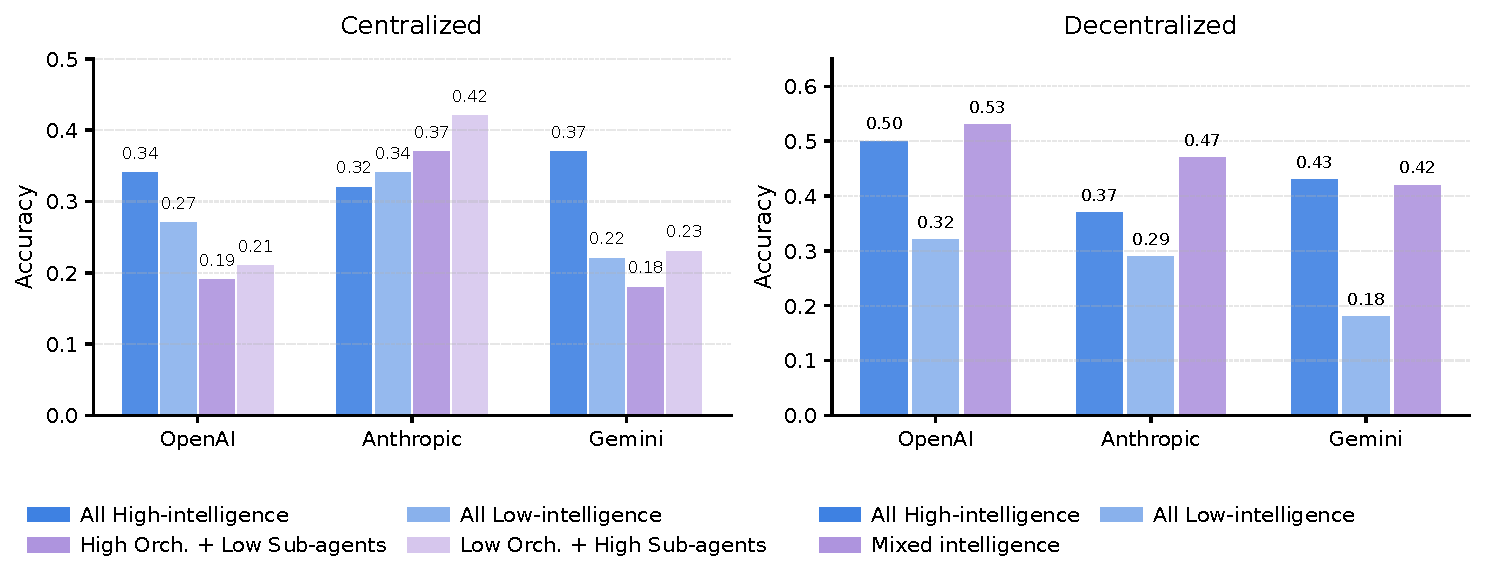
\includegraphics[width=\linewidth]{imgs/heterogeneous.pdf}
\caption{\textbf{Agent Heterogeneity Effects on Multi-Agent Performance.} 
Performance comparison of centralized (Orchestrator-Subagents) and decentralized (Peer Debate with Voting) multi-agent architectures on BrowseComp-Plus benchmark across three LLM families. High-capability models include GPT-5, Claude Sonnet 4.5, and Gemini-2.5 Pro; low-capability models include GPT-5 nano, Claude Sonnet 3.7, and Gemini-2.0 Flash.
(1) Anthropic models uniquely benefit from heterogeneous mixing in centralized architecture, where low-capability orchestrator with high-capability subagents (0.42) outperforms homogeneous high-capability (0.32) by 31\%, while OpenAI and Gemini show performance degradation under heterogeneous centralized configurations. 
(2) Decentralized mixed-capability approaches achieve near-optimal or superior performance compared to homogeneous high-capability baselines (OpenAI: 0.53 vs 0.50; Anthropic: 0.47 vs 0.37; Gemini: 0.42 vs 0.43), suggesting effective emergent collaboration despite capability asymmetry. 
(3) In centralized architectures, configurations with high-capability sub-agents outperform those with high-capability orchestrators across all model families, suggesting sub-agent capability matters more than orchestrator capability.}
    \label{fig:heterogeneous}
\end{figure}

  
\paragraph{Error Taxonomy Reveals Architecture-specific Failure Modes.}
We identified four error categories as follows.

(1) \textit{Logical Contradiction}: agent asserts both ``X is true'' and ``X is false'' about the same entity, or derives conclusions violating its stated premises;
(2) \textit{Numerical Drift}: accumulated computational error from cascading rounding or unit conversion mistakes, measured as relative deviation from ground truth exceeding 5\%;
(3) \textit{Context Omission}: failure to reference previously established entities, relationships, or state information required for the current reasoning step;
(4) \textit{Coordination Failure} (MAS-specific): message misinterpretation, task allocation conflicts, or state synchronization errors between agents. Architecture-specific patterns emerge across these categories:
\begin{itemize}[leftmargin=1.2em]
    \item \textbf{Logical Contradiction}: Baseline 12.3--18.7\%. Centralized reduces to 9.1\% (36.4\% reduction) via consensus; Decentralized achieves 11.5\% through peer verification; Independent unchanged at 16.8\%.
    
    \item \textbf{Numerical Drift}: Baseline 20.9--24.1\%. Centralized/Decentralized reduce to 18.3\% (24\% reduction) via sub-problem verification; Hybrid amplifies to 26.4\% as rounding errors propagate; Independent unchanged at 23.2\%.
    
    \item \textbf{Context Omission}: Baseline 15.8--25.2\%. Centralized reduces to 8.3\% (66.8\% reduction) via orchestrator synthesis; Decentralized achieves 11.2\%; Independent unchanged at 24.1\%.
    
    \item \textbf{Coordination Failure}: Only appears in MAS. Independent: 0\% (no coordination mechanism); Centralized: 1.8\%; Decentralized: 3.2\%; Hybrid: 12.4\% (protocol complexity exceeds robust implementation).
\end{itemize}
  
  These patterns identify three operational coordination regimes: (i) \textbf{Under-coordination} ($O < 100\%$ overhead): minimal accuracy gain ($\Delta S \approx +2$--4\%), coordination mechanisms not yet engaged; (ii) \textbf{Optimal band} ($200\% < O < 300\%$ overhead): highest success--cost ratio ($E_c \approx 0.16$), dominated by Centralized and Decentralized, with strong error absorption; (iii) \textbf{Over-coordination} ($O > 400\%$ overhead): Hybrid runs with reduced efficiency ($E_c \approx 0.11$), protocol complexity introducing coordination-failure modes. Error amplification analysis confirms: Independent architectures propagate errors to 17.2$\times$ baseline ($95\%$ CI: $[14.3, 20.1]$; no correction mechanisms), while Centralized contains to 4.4$\times$ ($[3.8, 5.0]$) through supervised aggregation.
  
  

\begin{figure}[t]
\centering
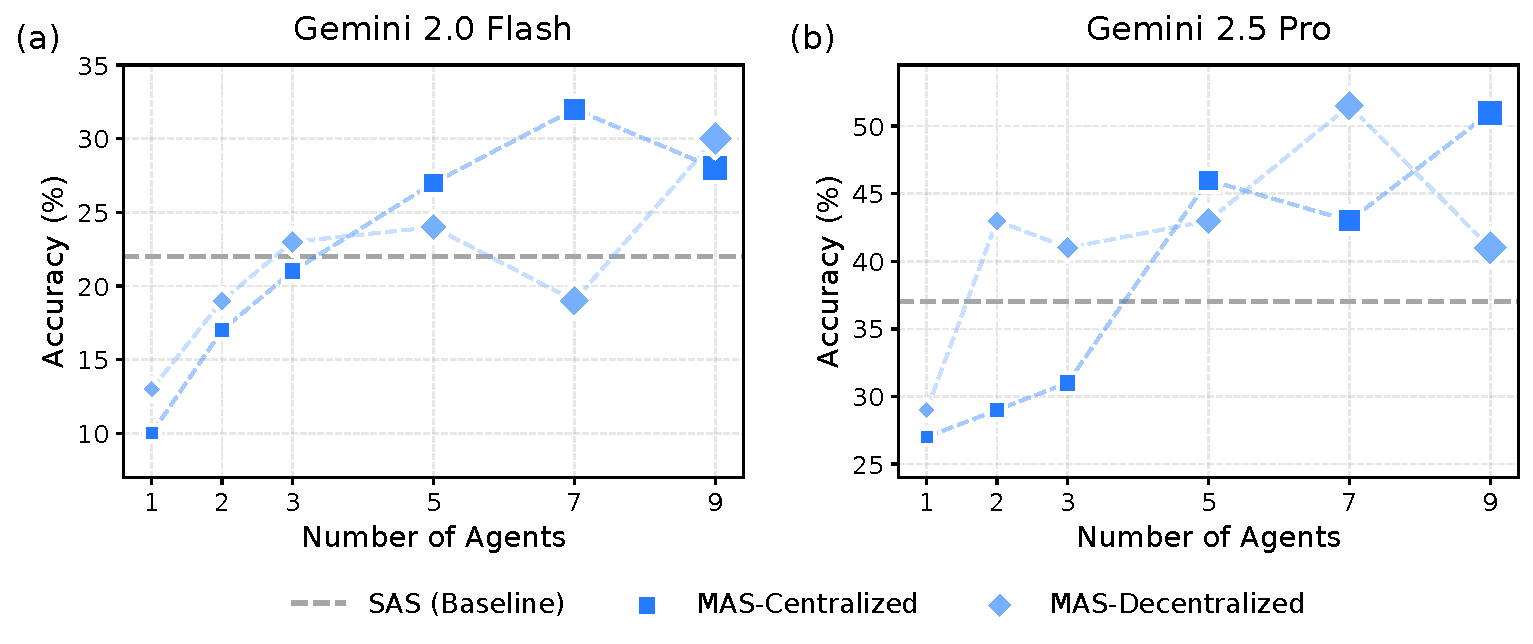
\includegraphics[width=0.85\textwidth]{imgs/architecture_comparison_combined.pdf}
\caption{\textbf{Number of agents scaling reveals model-dependent coordination limits.} Performance of Gemini-2.0 Flash (\textbf{a}) and Gemini-2.5 Pro (\textbf{b}) across multi-agent architectures with varying number of agents ($n_a \in \{1, 3, 5, 7, 9\}$). Both models show initial 
gains from multi-agent coordination, but scaling patterns diverge: 
Gemini-2.0 Flash exhibits a clear optimum at 7 agents before degradation, while Gemini-2.5 Pro's decentralized architecture peaks earlier despite its higher single-agent baseline. The centralized architecture demonstrates more stable scaling for Flash but shows diminishing returns for Pro beyond 5 agents. Dashed lines indicate single-agent baseline performance. Results suggest that the optimal number of agents depends on both model capacity and coordination strategy, with coordination overhead eventually outweighing parallelization 
benefits.}
\label{fig:agent_scaling}
\end{figure}
  

\paragraph{Information Gain (IG) Predicts MAS benefit in Low-Complexity Domains.}
  We compute information gain $\Delta \mathcal{I}$ by comparing pre-coordination and post-coordination task-uncertainty surrogates (via Bayesian posterior variance reduction on key variables). In structured domains (Finance Agent, Workbench), $\Delta \mathcal{I}$ correlates strongly with MAS--SAS gap ($r = 0.71$, $p < 0.001$), indicating that agents successfully exchange high-value information and synthesize it into improved solutions. In Finance Agent specifically, $\Delta \mathcal{I}$ ranges 0.8--2.1 bits (mean 1.4) for successful trials vs.\ 0.2--0.6 bits (mean 0.4) for failures.
  
  Conversely, in open-world domains (BrowseComp-Plus), $\Delta \mathcal{I}$ shows weak and non-significant power, revealing that agents' messages provide limited validated information due to inherent world ambiguity. This domain-dependent information-gain pattern directly maps to observed MAS benefits: Finance Agent (up to +80.8\% for Centralized) where information exchange is high-value; BrowseComp-Plus (up to +9.2\% for Decentralized) where world ambiguity limits verification.
  
  \paragraph{Cross-Domain Consistency of Coordination Patterns.}
  Architectural rankings remained stable across domains (Kendall $\tau = 0.89$, coefficient of variation $< 0.1$ across architectures), indicating coordination principles transcend specific task structures. \textcolor{black}{Extrapolation to larger teams via the fitted power law predicts $\approx$69 turns at $n{=}6$ and $\approx$157 turns at $n{=}10$ (95\% CI from exponent uncertainty: [64, 74] and [143, 172] respectively), corresponding to $9.5\times$--$21.8\times$ increases over the SAS baseline of 7.2 turns.} This super-linear scaling confirms the hard resource ceiling: beyond 3--4 agents, per-agent reasoning quality degrades sharply under fixed budgets.
  
  \paragraph{Economic Efficiency and Family-Specific Cost-Benefit Trade-offs.}
  Token efficiency (success per 1,000 tokens) reveals sharp trade-offs by architecture and family: SAS achieves 67.7 successes/1K tokens; Centralized drops to 21.5 (3.1$\times$ worse); Decentralized to 23.9 (2.8$\times$ worse); Hybrid to 13.6 (5.0$\times$ worse). Absolute dollar costs per trial vary by model: OpenAI Hybrid achieves marginal cost $\approx\$0.008$ per 1\% success gain (steep but manageable for structured tasks), while Anthropic Hybrid reaches $\approx\$0.024$ per 1\% gain (3$\times$ worse, reflecting Anthropic's sensitivity to coordination overhead). Google maintains intermediate costs $\approx\$0.012$ per 1\% gain across architectures, suggesting more balanced cost-benefit trade-offs.
  
  \paragraph{LLM Family-specific Deployment Signatures and Model-Architecture Alignment.}
  Cross-family analysis reveals distinct architectural preferences. OpenAI models show strongest Hybrid gains on structured tasks (Finance: 52\% success Hybrid vs.\ 39\% SAS; Workbench: 56\% Hybrid vs.\ 42\% SAS). Anthropic models display most conservative, stable Centralized performance (mean 43\% across tasks, SD = 2.3\%, lowest variance). Google models exhibit consistent cross-architecture efficiency (performance range < 5\% across topologies). These patterns may reflect family-level differences in instruction following, context utilization, inter-turn consistency, or other architectural and training factors that affect how models process coordination messages. We do not isolate the underlying mechanism here, so these family-specific differences should be interpreted as empirical signatures rather than mechanistic conclusions.

\textcolor{black}{
\subsection{Robustness and Sensitivity Analysis}
\label{subsec:extended_validation}
We subject the 6-benchmark regression ($N=260$) to three robustness checks addressing pseudoreplication, multiplicity, and capability metric sensitivity.
\paragraph{Cluster-robust inference.} We re-estimated the regression with cluster-robust standard errors (clustering on dataset, $G=6$, CR1 correction, $t_5$ critical values). Predictors varying primarily at the dataset level (including \texttt{log\_tools}, \texttt{efficiency\_x\_tools}, and \texttt{baseline\_x\_agents}) show standard error inflation up to $2.9\times$ relative to naive OLS estimates; we report these as directional patterns rather than confirmed effects. \texttt{single\_agent\_baseline} ($p=0.004$) and \texttt{error\_x\_baseline} ($p=0.030$) retain significance under cluster-robust inference, confirming the capability-saturation finding as the most robustly supported result (Table~\ref{tab:s4_cluster}).
\paragraph{Multiple-comparison correction.} We evaluated 19 predictor coefficients (excluding the intercept) as a single family of simultaneous hypotheses, applying the Holm--Bonferroni step-down procedure to control the family-wise error rate at $\alpha=0.05$. Three predictors survive correction: \texttt{log\_tools} ($p_{\text{Holm}}<0.001$), \texttt{single\_agent\_baseline} ($p_{\text{Holm}}=0.018$), and \texttt{efficiency\_x\_tools} ($p_{\text{Holm}}=0.026$). Two further predictors (\texttt{intelligence\_centered} and \texttt{baseline\_x\_agents}) are suggestive ($p_{\text{Holm}}<0.10$) and are discussed as directional patterns (Table~\ref{tab:s5_holm}). The Holm--Bonferroni correction was applied to naive OLS $p$-values (addressing multiplicity), while the cluster-robust analysis (addressing pseudoreplication) was reported separately. Under cluster-robust inference alone, only \texttt{single\_agent\_baseline} ($p=0.004$) survives at $\alpha=0.05$, making capability saturation the single most robust finding across both correction approaches.
\paragraph{Capability metric sensitivity.} As an alternative to the Intelligence Index, we introduce the Agentic Capability Index (ACI), defined as each model's mean single-agent performance across all six benchmarks. The two metrics are only moderately correlated ($r = 0.45$), validating the concern that static benchmark composites diverge from dynamic agentic performance. ACI improves cross-validated fit ($R^2_{\text{CV}}$: $0.373 \to 0.413$) with zero finding reversals, and we recommend ACI as the primary capability metric going forward (Table~\ref{tab:s3_aci}).
\paragraph{Cross-domain generalization.} 
Leave-one-dataset-out (LODO) cross-validation highlights the challenge of predicting \emph{absolute} success rates across structurally diverse task domains with a single regression surface that contains no dataset-specific parameters. 
However, within-domain cross-validated evaluation shows that the model correctly identifies the optimal architecture for 87\% of held-out configurations (\S\ref{subsec:scaling}), indicating that \emph{relative} performance rankings between architectures are preserved even when absolute cross-domain prediction is limited. 
The capability-saturation threshold ($\sim$45\%) is further supported with a 94\% match rate across all 16 model$\times$benchmark configurations on SWE-bench Verified and Terminal-Bench ($p < 0.001$ by binomial test).
}

